\addcontentsline{toc}{chapter}{Micah}

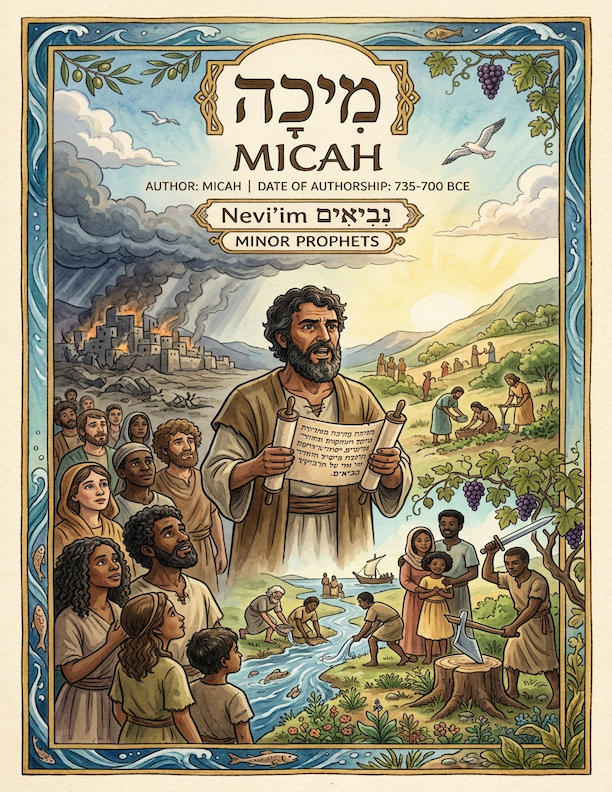
\includepdf[pages=1, fitpaper=false, width=\paperwidth, height=\paperheight, , keepaspectratio=false]{images/divider2/micah_2.png}
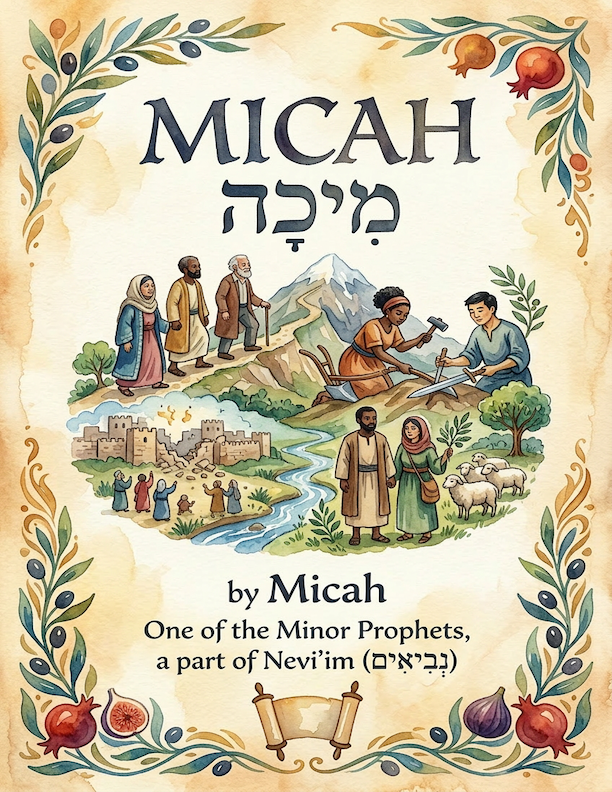
\includepdf[pages=1, fitpaper=false, width=\paperwidth, height=\paperheight, , keepaspectratio=false]{images/divider1/micah.png}

\includepdf[pages=1, fitpaper=false, width=\paperwidth, height=\paperheight, , keepaspectratio=false]{images/8.5x11-Dot-Grid.png}

\includepdf[pages=1, fitpaper=false, width=\paperwidth, height=\paperheight, , keepaspectratio=false]{images/8.5x11-Dot-Grid.png}
\mybook{Micah}
\vspace{-1.36in}
\begin{multicols}{2}
\mychapter{} \myverse*{}The LORD’s\footnote{1:1 When rendered in ALL CAPITAL LETTERS, “LORD” or “GOD” is the translation of God’s Proper Name.}
word that came to Micah of Morasheth in the days of Jotham, Ahaz, and Hezekiah, kings of Judah, which
he saw concerning Samaria and Jerusalem.

\myverse{}Hear, you peoples, all of you!

Listen, O earth, and all that is therein.

Let the Lord\footnote{1:2 The word translated “Lord” (mixed case) is “Adonai.”} GOD be witness against you,

the Lord from his holy temple.

\myverse{}For behold,\footnote{1:3 “Behold”, from “הִנֵּה”, means look at, take notice, observe, see, or gaze at. It is
	often used as an interjection.} the LORD comes out of his place,

and will come down and tread on the high places of the earth.

\myverse{}The mountains melt under him,

and the valleys split apart like wax before the fire,

like waters that are poured down a steep place.


\vspace{\baselineskip} \myverse{}“All this is for the disobedience of Jacob,

and for the sins of the house of Israel.

What is the disobedience of Jacob?

Isn’t it Samaria?

And what are the high places of Judah?

Aren’t they Jerusalem?

\myverse{}Therefore I will make Samaria like a rubble heap of the field,

like places for planting vineyards;

and I will pour down its stones into the valley,

and I will uncover its foundations.

\myverse{}All her idols will be beaten to pieces,

all her temple gifts will be burned with fire,

and I will destroy all her images;

for of the hire of a prostitute has she gathered them,

and to the hire of a prostitute shall they return.”


\vspace{\baselineskip} \myverse{}For this I will lament and wail.

I will go stripped and naked.

I will howl like the jackals

and mourn like the ostriches.

\myverse{}For her wounds are incurable;

for it has come even to Judah.

It reaches to the gate of my people,

even to Jerusalem.

\myverse{}Don’t tell it in Gath.

Don’t weep at all.

At Beth Ophrah\footnote{1:10 Beth Ophrah means literally “House of Dust.”} I have rolled myself in the dust.

\myverse{}Pass on, inhabitant of Shaphir, in nakedness and shame.

The inhabitant of Zaanan won’t come out.

The wailing of Beth Ezel will take from you his protection.

\myverse{}For the inhabitant of Maroth waits anxiously for good,

because evil has come down from the LORD to the gate of Jerusalem.

\myverse{}Harness the chariot to the swift steed, inhabitant of Lachish.

She was the beginning of sin to the daughter of Zion;

for the transgressions of Israel were found in you.

\myverse{}Therefore you will give a parting gift to Moresheth Gath.

The houses of Achzib will be a deceitful thing to the kings of Israel.

\myverse{}I will yet bring a conqueror to you, inhabitants of Mareshah.

The glory of Israel will come to Adullam.

\myverse{}Shave your heads,

and cut off your hair for the children of your delight.

Enlarge your baldness like the vulture,

for they have gone into captivity from you!


%MICAH 2
\mychapter{} \myverse*{}Woe to those who devise iniquity

and work evil on their beds!

When the morning is light, they practice it,

because it is in the power of their hand.

\myverse{}They covet fields and seize them,

and houses, then take them away.

They oppress a man and his house,

even a man and his heritage.

\myverse{}Therefore the LORD says:

“Behold, I am planning against these people a disaster,

from which you will not remove your necks,

neither will you walk haughtily,

for it is an evil time.

\myverse{}In that day they will take up a parable against you,

and lament with a doleful lamentation, saying,

‘We are utterly ruined!

My people’s possession is divided up.

Indeed he takes it from me and assigns our fields to traitors!’ ”

\myverse{}Therefore you will have no one who divides the land by lot in
the LORD’s assembly.

\myverse{}“Don’t prophesy!”—they prophesy—

“Don’t prophesy about these things.

Disgrace won’t overtake us.”

\myverse{}Shall it be said, O house of Jacob,

“Is the LORD’s Spirit angry?

Are these his doings?

Don’t my words do good to him who walks blamelessly?”

\myverse{}But lately my people have risen up as an enemy.

You strip the robe and clothing from those who pass by without a care, returning
from battle.

\myverse{}You drive the women of my people out from their pleasant houses;

from their young children you take away my blessing forever.

\myverse{}Arise, and depart!

For this is not your resting place,

because of uncleanness that destroys,

even with a grievous destruction.

\myverse{}If a man walking in a spirit of falsehood lies, saying,

“I will prophesy to you of wine and of strong drink,”

he would be the prophet of this people.

\myverse{}I will surely assemble all of you, Jacob.

I will surely gather the remnant of Israel.

I will put them together as the sheep of Bozrah,

as a flock in the middle of their pasture.

They will swarm with people.

\myverse{}He who breaks open the way goes up before them.

They break through the gate, and go out.

Their king passes on before them,

with the LORD at their head.


%MICAH 3
\mychapter{} \myverse*{}I said,

“Please listen, you heads of Jacob,

and rulers of the house of Israel:

Isn’t it for you to know justice?

\myverse{}You who hate the good,

and love the evil;

who tear off their skin,

and their flesh from off their bones;

\myverse{}who also eat the flesh of my people,

and peel their skin from off them,

and break their bones,

and chop them in pieces, as for the pot,

and as meat within the cauldron.

\myverse{}Then they will cry to the LORD,

but he will not answer them.

Yes, he will hide his face from them at that time,

because they made their deeds evil.”

\myverse{}The LORD says concerning the prophets who lead my people astray—for
those who feed their teeth, they proclaim, “Peace!” and whoever doesn’t provide for their mouths, they
prepare war against him:

\myverse{}“Therefore night is over you, with no vision,

and it is dark to you, that you may not divine;

and the sun will go down on the prophets,

and the day will be black over them.

\myverse{}The seers shall be disappointed,

and the diviners confounded.

Yes, they shall all cover their lips,

for there is no answer from God.”\footnote{3:7 The Hebrew word rendered “God” is “אֱלֹהִ֑ים” (Elohim).}

\myverse{}But as for me, I am full of power by the LORD’s Spirit,

and of judgment, and of might,

to declare to Jacob his disobedience,

and to Israel his sin.

\myverse{}Please listen to this, you heads of the house of Jacob,

and rulers of the house of Israel,

who abhor justice,

and pervert all equity,

\myverse{}who build up Zion with blood,

and Jerusalem with iniquity.

\myverse{}Her leaders judge for bribes,

and her priests teach for a price,

and her prophets of it tell fortunes for money;

yet they lean on the LORD, and say,

“Isn’t the LORD among us?

No disaster will come on us.”

\myverse{}Therefore Zion for your sake will be plowed like a field,

and Jerusalem will become heaps of rubble,

and the mountain of the temple like the high places of a forest.


%MICAH 4
\mychapter{} \myverse*{}But in the latter days,

it will happen that the mountain of the LORD’s temple will be established on the
top of the mountains,

and it will be exalted above the hills;

and peoples will stream to it.

\myverse{}Many nations will go and say,

“Come! Let’s go up to the mountain of the LORD,

and to the house of the God of Jacob;

and he will teach us of his ways,

and we will walk in his paths.”

For the law will go out of Zion,

and the LORD’s word from Jerusalem;

\myverse{}and he will judge between many peoples,

and will decide concerning strong nations afar off.

They will beat their swords into plowshares,

and their spears into pruning hooks.

Nation will not lift up sword against nation,

neither will they learn war any more.

\myverse{}But every man will sit under his vine and under his fig tree.

No one will make them afraid,

for the mouth of the LORD of Hosts has spoken.
\myverse{}Indeed all the nations may walk in the name of their gods,

but we will walk in the name of the LORD our God forever and ever.

\myverse{}“In that day,” says the LORD,

“I will assemble that which is lame,

and I will gather that which is driven away,

and that which I have afflicted;

\myverse{}and I will make that which was lame a remnant,

and that which was cast far off a strong nation:

and the LORD will reign over them on Mount Zion from then on, even forever.”

\myverse{}You, tower of the flock, the hill of the daughter of Zion,

to you it will come.

Yes, the former dominion will come,

the kingdom of the daughter of Jerusalem.


\vspace{\baselineskip} \myverse{}Now why do you cry out aloud?

Is there no king in you?

Has your counselor perished,

that pains have taken hold of you as of a woman in travail?

\myverse{}Be in pain, and labor to give birth, daughter of Zion,

like a woman in travail;

for now you will go out of the city,

and will dwell in the field,

and will come even to Babylon.

There you will be rescued.

There the LORD will redeem you from the hand of your enemies.


\vspace{\baselineskip} \myverse{}Now many nations have assembled against you, that say,

“Let her be defiled,

and let our eye gloat over Zion.”

\myverse{}But they don’t know the thoughts of the LORD,

neither do they understand his counsel;

for he has gathered them like the sheaves to the threshing floor.

\myverse{}Arise and thresh, daughter of Zion,

for I will make your horn iron,

and I will make your hoofs bronze.

You will beat in pieces many peoples.

I will devote their gain to the LORD,

and their substance to the Lord of the whole earth.

%MICAH 5
\mychapter{} \myverse*{}Now you shall gather yourself in troops,

daughter of troops.

He has laid siege against us.

They will strike the judge of Israel with a rod on the cheek.

\myverse{}But you, Bethlehem Ephrathah,

being small among the clans of Judah,

out of you one will come out to me who is to be ruler in Israel;

whose goings out are from of old, from ancient times.

\myverse{}Therefore he will abandon them until the time that she who is
in labor gives birth.

Then the rest of his brothers will return to the children of Israel.

\myverse{}He shall stand, and shall shepherd in the strength of the LORD,

in the majesty of the name of the LORD his God.

They will live, for then he will be great to the ends of the earth.

\myverse{}He will be our peace when Assyria invades our land

and when he marches through our fortresses,

then we will raise against him seven shepherds,

and eight leaders of men.

\myverse{}They will rule the land of Assyria with the sword,

and the land of Nimrod in its gates.

He will deliver us from the Assyrian,

when he invades our land,

and when he marches within our border.

\myverse{}The remnant of Jacob will be among many peoples

like dew from the LORD,

like showers on the grass,

that don’t wait for man

nor wait for the sons of men.

\myverse{}The remnant of Jacob will be among the nations,

among many peoples,

like a lion among the animals of the forest,

like a young lion among the flocks of sheep;

who, if he goes through, treads down and tears in pieces,

and there is no one to deliver.

\myverse{}Let your hand be lifted up above your adversaries,

and let all of your enemies be cut off.

\myverse{}“It will happen in that day”, says the LORD,

“that I will cut off your horses from among you

and will destroy your chariots.

\myverse{}I will cut off the cities of your land

and will tear down all your strongholds.

\myverse{}I will destroy witchcraft from your hand.

You shall have no soothsayers.

\myverse{}I will cut off your engraved images and your pillars from among
you;

and you shall no more worship the work of your hands.

\myverse{}I will uproot your Asherah poles from among you;

and I will destroy your cities.

\myverse{}I will execute vengeance in anger

and wrath on the nations that didn’t listen.”


%MICAH 6
\mychapter{} \myverse*{}Listen now to what the LORD says:

“Arise, plead your case before the mountains,

and let the hills hear what you have to say.

\myverse{}Hear, you mountains, the LORD’s indictment,

and you enduring foundations of the earth;

for the LORD has a case against his people,

and he will contend with Israel.

\myverse{}My people, what have I done to you?

How have I burdened you?

Answer me!

\myverse{}For I brought you up out of the land of Egypt,

and redeemed you out of the house of bondage.

I sent before you Moses, Aaron, and Miriam.

\myverse{}My people, remember now what Balak king of Moab devised,

and what Balaam the son of Beor answered him from Shittim to Gilgal,

that you may know the righteous acts of the LORD.”


\vspace{\baselineskip} \myverse{}How shall I come before the LORD,

and bow myself before the exalted God?

Shall I come before him with burnt offerings,

with calves a year old?

\myverse{}Will the LORD be pleased with thousands of rams?

With tens of thousands of rivers of oil?

Shall I give my firstborn for my disobedience?

The fruit of my body for the sin of my soul?

\myverse{}He has shown you, O man, what is good.

What does the LORD require of you, but to act justly,

to love mercy, and to walk humbly with your God?


\vspace{\baselineskip} \myverse{}The LORD’s voice calls to the city—

and wisdom fears your name—

“Listen to the rod,

and he who appointed it.

\myverse{}Are there yet treasures of wickedness in the house of the wicked,

and a short efah\footnote{6:10 An efah is a measure of volume (about 22 liters or about 2/3 of a bushel), and a short efah is
	made smaller than a full efah for the purpose of cheating customers.} that is accursed?

\myverse{}Shall I tolerate dishonest scales,

and a bag of deceitful weights?

\myverse{}Her rich men are full of violence,

her inhabitants speak lies,

and their tongue is deceitful in their speech.

\myverse{}Therefore I also have struck you with a grievous wound.

I have made you desolate because of your sins.

\myverse{}You shall eat, but not be satisfied.

Your hunger will be within you.

You will store up, but not save,

and that which you save I will give up to the sword.

\myverse{}You will sow, but won’t reap.

You will tread the olives, but won’t anoint yourself with oil;

and crush grapes, but won’t drink the wine.

\myverse{}For the statutes of Omri are kept,

and all the works of Ahab’s house.

You walk in their counsels,

that I may make you a ruin,

and your inhabitants a hissing.

You will bear the reproach of my people.”

%MICAH 7
\mychapter{} \myverse*{}Misery is mine!

Indeed, I am like one who gathers the summer fruits, as gleanings of the vineyard.

There is no cluster of grapes to eat.

My soul desires to eat the early fig.

\myverse{}The godly man has perished out of the earth,

and there is no one upright among men.

They all lie in wait for blood;

every man hunts his brother with a net.

\myverse{}Their hands are on that which is evil to do it diligently.

The ruler and judge ask for a bribe.

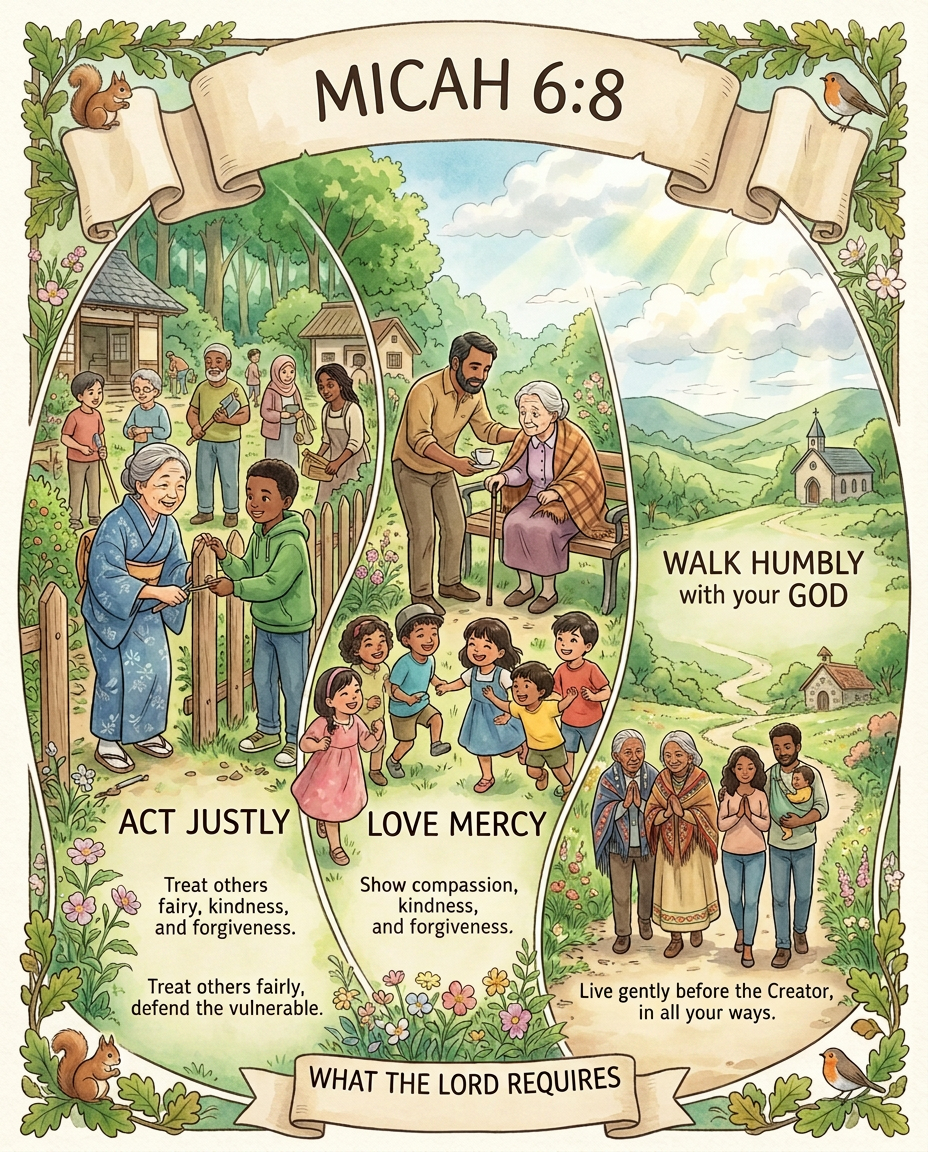
\includepdf[pages=1, fitpaper=false, width=\paperwidth, height=\paperheight, , keepaspectratio=false]{micah-6-8.png}

\noindent The powerful man dictates the evil desire of his soul.

Thus they conspire together.

\myverse{}The best of them is like a brier.

The most upright is worse than a thorn hedge.

The day of your watchmen,

even your visitation, has come;

now is the time of their confusion.

\myverse{}Don’t trust in a neighbor.

Don’t put confidence in a friend.

With the woman lying in your embrace,

be careful of the words of your mouth!

\myverse{}For the son dishonors the father,

the daughter rises up against her mother,

the daughter-in-law against her mother-in-law;

a man’s enemies are the men of his own house.

\myverse{}But as for me, I will look to the LORD.

I will wait for the God of my salvation.

My God will hear me.

\myverse{}Don’t rejoice against me, my enemy.

When I fall, I will arise.

When I sit in darkness, the LORD will be a light to me.

\myverse{}I will bear the indignation of the LORD,

because I have sinned against him,

until he pleads my case and executes judgment for me.

He will bring me out to the light.

I will see his righteousness.

\myverse{}Then my enemy will see it,

and shame will cover her who said to me,

“Where is the LORD your God?”

My eyes will see her.

Now she will be trodden down like the mire of the streets.

\myverse{}A day to build your walls!

In that day, he will extend your boundary.

\myverse{}In that day they will come to you from Assyria and the cities
of Egypt,

and from Egypt even to the River,

and from sea to sea,

and mountain to mountain.

\myverse{}Yet the land will be desolate because of those who dwell therein,

for the fruit of their doings.

\myverse{}Shepherd your people with your staff,

the flock of your heritage,

who dwell by themselves in a forest.

Let them feed in the middle of fertile pasture land,

in Bashan and Gilead, as in the days of old.

\myverse{}“As in the days of your coming out of the land of Egypt,

I will show them marvelous things.”

\myverse{}The nations will see and be ashamed of all their might.

They will lay their hand on their mouth.

Their ears will be deaf.

\myverse{}They will lick the dust like a serpent.

Like crawling things of the earth, they will come trembling out of their dens.

They will come with fear to the LORD our God,

and will be afraid because of you.

\myverse{}Who is a God like you, who pardons iniquity,

and passes over the disobedience of the remnant of his heritage?

He doesn’t retain his anger forever,

because he delights in loving kindness.

\myverse{}He will again have compassion on us.

He will tread our iniquities under foot.

You will cast all their sins into the depths of the sea.

\myverse{}You will give truth to Jacob,

and mercy to Abraham,

as you have sworn to our fathers from the days of old.
\end{multicols}
